\chapter{Matematiske Forutsetninger}
\label{chap:preliminaries}

\section{Lineær algebra}

\subsection{Jordan form}
\gls{jordan}-formen er en kanonisk form som enhver kompleks matrise kan bringes til ved en similaritatstransformasjon.

Denne formen er spesielt nyttig når matrisen ikke er diagonaliserbar, og gir oss en elegant måte å forstå matrisens struktur og oppførsel.

\begin{definition}{Jordan-form}{jordan_form}
	La $A \in \mathbb{C}^{n \times n}$ være en matrise. Det finnes en invertibel matrise $P$ slik at $P^{-1}AP = J$ hvor $J$ er på Jordan-form, dvs.
	\[
		J =
		\begin{pmatrix}
			J_1 &     &        &     \\
			    & J_2 &        &     \\
			    &     & \ddots &     \\
			    &     &        & J_k
		\end{pmatrix}
	\]
	hvor hver $J_i$ er en Jordan-blokk med formen
	\[
		J_i =
		\begin{pmatrix}
			\lambda_i & 1         &        &           \\
			          & \lambda_i & \ddots &           \\
			          &           & \ddots & 1         \\
			          &           &        & \lambda_i
		\end{pmatrix}
	\]
	der $\lambda_i$ er en egenverdi av $A$.
\end{definition}

\begin{remark}{Jordan-blokker}{jordan_blocks}
	Jordan-blokkene representerer hvordan $A$ virker på generaliserte egenvektorer.

	En Jordan-blokk av størrelse $m$ med egenverdi $\lambda$ tilsvarer en kjede av $m$ generaliserte egenvektorer $v_1, v_2, \ldots, v_m$ som oppfyller
	\[
		(A - \lambda I)v_1 = 0, \quad (A - \lambda I)v_2 = v_1, \quad \ldots, \quad (A - \lambda I)v_m = v_{m-1}
	\]
	Dette viser hvordan matrisen "kobler sammen" vektorer i sin virkning.
\end{remark}

\begin{example}{Jordan-form av en \(3 \times 3\) matrise}{jordan_example}
	La
	\[
		A = \begin{pmatrix} 3 & 1 & 0 \\ 1 & 3 & 0 \\ 0 & 0 & 2 \end{pmatrix}
	\]
	Denne matrisen har egenverdi $\lambda_1 = 4$ med algebraisk og geometrisk multiplisitet 1, egenverdi $\lambda_2 = 2$ med algebraisk multiplisitet 2 og geometrisk multiplisitet 1. Vi kan beregne transformasjonsmatrisen $P$ og få Jordanformen:
	\[
		J = P^{-1}AP = \begin{pmatrix} 4 & 0 & 0 \\ 0 & 2 & 1 \\ 0 & 0 & 2 \end{pmatrix}
	\]
	med en $1 \times 1$ Jordan-blokk for $\lambda_1 = 4$ og en $2 \times 2$ Jordan-blokk for $\lambda_2 = 2$.
\end{example}

\begin{figure}
	\centering
	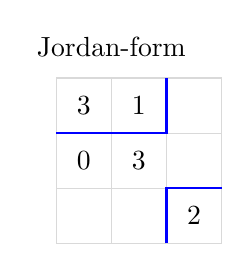
\begin{tikzpicture}
		% Jordan blocks grid
		\draw[step=0.7cm,color=gray!30] (0,0) grid (2.1,2.1);

		% Jordan block 1 (2x2)
		\node at (0.35,1.75) {$3$};
		\node at (1.05,1.75) {$1$};
		\node at (0.35,1.05) {$0$};
		\node at (1.05,1.05) {$3$};

		% Jordan block 2 (1x1)
		\node at (1.75,0.35) {$2$};

		% Draw boundaries
		\draw[blue,thick] (0,1.4) -- (1.4,1.4) -- (1.4,2.1);
		\draw[blue,thick] (1.4,0) -- (1.4,0.7) -- (2.1,0.7);

		% Labels
		\node at (0.7,2.5) {Jordan-form};
	\end{tikzpicture}
	\caption{Visualisering av Jordan-form med to Jordan-blokker. De blå linjene indikerer grensene mellom de forskjellige Jordan-blokkene.}
	\label{fig:jordan_form}
\end{figure}

\subsubsection{Geometrisk tolkning av Jordan-form}
En Jordan-blokk med egenverdi $\lambda$ representerer en transformasjon med to effekter:
\begin{itemize}
	\item \textbf{Skalering}: Egenvektorer strekkes/komprimeres med faktor $\lambda$
	\item \textbf{Skjæring}: Generaliserte egenvektorer forskyves i retning av egenvektorer med lavere rang, i tillegg til å skaleres
\end{itemize}

Denne tolkningen gjør det lettere å forstå hvordan en ikke-diagonaliserbar matrise oppfører seg geometrisk.

\begin{figure}[H]
	\centering
	\begin{tikzpicture}
		% Coordinate system
		\draw[->] (-3,0) -- (3,0) node[right] {$x$};
		\draw[->] (0,-3) -- (0,3) node[above] {$y$};

		% Original vectors
		\draw[->,thick,blue] (0,0) -- (1,0) node[midway,below] {$v_1$};
		\draw[->,thick,red] (0,0) -- (0,1) node[midway,left] {$v_2$};

		% Transformed vectors (assuming lambda = 2)
		\draw[->,thick,blue,dashed] (0,0) -- (2,0) node[midway,above] {$Av_1$};
		\draw[->,thick,red,dashed] (0,0) -- (1,2) node[midway,right] {$Av_2$};

		% Arrow showing the shear effect
		\draw[->,thick,red,dotted] (0,2) -- (1,2);

		\node at (2,2) {\(J = \begin{pmatrix} 2 & 1 \\ 0 & 2 \end{pmatrix}\)};
		\node at (0,-3.5) {\(\lambda = 2\)};
	\end{tikzpicture}
	\caption{Geometrisk illustrasjon av en $2 \times 2$ Jordan-blokk med $\lambda = 2$. $v_1$ er en egenvektor som kun skaleres, mens $v_2$ er en generalisert egenvektor som både skaleres og forskyves i $v_1$-retningen.}
	\label{fig:jordan_action}
\end{figure}

\subsection{Symmetriske matriser}
Symmetriske matriser spiller en spesielt viktig rolle i anvendelser på grunn av deres fine egenskaper.

\begin{definition}{Symmetrisk matrise}{symmetric_matrix}
	En matrise $A \in \mathbb{R}^{n \times n}$ er symmetrisk hvis $A = A^T$, det vil si at $a_{ij} = a_{ji}$ for alle $i,j$.
\end{definition}

Symmetriske matriser har flere viktige egenskaper som gjør dem spesielt nyttige i numeriske beregninger:

\begin{theorem}{Spektralteoremet for symmetriske matriser}{spectral_theorem}
	Hvis $A \in \mathbb{R}^{n \times n}$ er symmetrisk, så er $A$ ortogonalt diagonaliserbar. Det vil si at det finnes en ortogonal matrise $Q$ ($Q^T Q = I$) slik at
	\[
		Q^T A Q = \Lambda = \text{diag}(\lambda_1, \lambda_2, \ldots, \lambda_n)
	\]
	hvor $\lambda_1, \lambda_2, \ldots, \lambda_n$ er egenverdiene til $A$.

	Dessuten er alle egenverdiene til $A$ reelle, og egenvektorer som tilhører forskjellige egenverdier er ortogonale.
\end{theorem}

Dette teoremet forteller oss at symmetriske matriser har spesielt fine egenskaper: reelle egenverdier og ortogonale egenvektorer. Dette gjør dem ideelle for mange anvendelser innen numerisk analyse og fysikk.

\begin{figure}
	\centering
	\begin{tikzpicture}
		% Original circle
		\draw[blue] (0,0) circle (1cm);

		% Coordinate axes
		\draw[->] (-2.5,0) -- (2.5,0) node[right] {$x$};
		\draw[->] (0,-2.5) -- (0,2.5) node[above] {$y$};

		% Eigenvectors
		\draw[->, thick, red] (0,0) -- (1.5, 0) node[right] {$v_1$};
		\draw[->, thick, red] (0,0) -- (0, 1) node[above] {$v_2$};

		% Transformed circle (using eigenvalues 2 and 0.5)
		\draw[blue, dashed] (0,0) ellipse (2cm and 0.5cm);

		\node at (0,-2) {Symmetrisk transformasjon: $A = \begin{pmatrix} 2 & 0 \\ 0 & 0.5 \end{pmatrix}$};
	\end{tikzpicture}
	\caption{Virkningen av en symmetrisk matrise på en sirkel. Transformasjonen strekker og komprimerer kun langs ortogonale akser (egenvektorene), uten rotasjon eller skjæring.}
	\label{fig:symmetric_action}
\end{figure}

\subsection{Positiv definitte matriser}
Positiv definitte matriser er en spesiell type symmetriske matriser som dukker opp i mange anvendelser, særlig i optimalisering, statistikk og differensialligninger.

\begin{definition}{Positiv definitt matrise}{positive_definite}
	En symmetrisk matrise $A \in \mathbb{R}^{n \times n}$ er positiv definitt hvis
	\[
		x^T A x > 0 \quad \text{for alle } x \in \mathbb{R}^n, x \neq 0
	\]
	A er positiv semidefinitt hvis $x^T A x \geq 0$ for alle $x \in \mathbb{R}^n$.
\end{definition}

Intuitivt betyr dette at en positiv definitt matrise "peker" enhver vektor i en retning som gir en positiv projeksjon på den opprinnelige vektoren.

\begin{theorem}{Ekvivalente betingelser for positiv definitthet}{pd_equivalence}
	Følgende betingelser er ekvivalente for en symmetrisk matrise $A \in \mathbb{R}^{n \times n}$:
	\begin{enumerate}
		\item $A$ er positiv definitt.
		\item Alle egenverdiene til $A$ er positive.
		\item Alle hovedminorene til $A$ er positive (Sylvesters kriterium).
		\item $A = B^T B$ for en matrise $B$ med full kolonnerang.
		\item Det finnes en unik positiv definitt matrise $C$ slik at $C^2 = A$ (den positive kvadratroten).
	\end{enumerate}
\end{theorem}

Disse ekvivalente betingelsene gir oss flere praktiske måter å sjekke om en matrise er positiv definitt.

\begin{figure}[H]
	\centering
	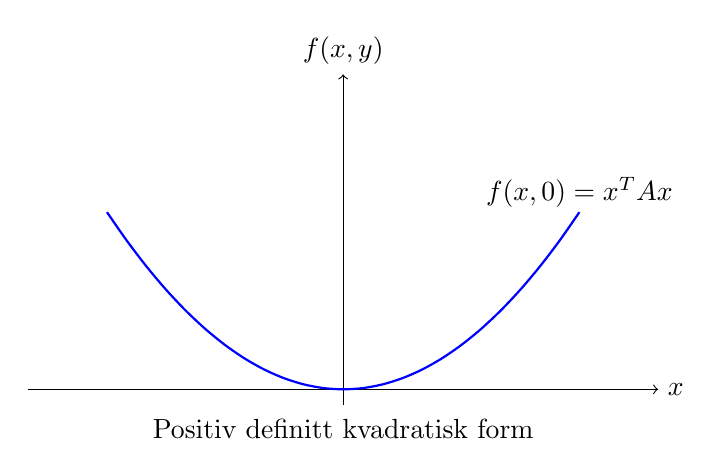
\begin{tikzpicture}
		% Coordinate system
		\draw[->] (-4,0) -- (4,0) node[right] {$x$};
		\draw[->] (0,-0.2) -- (0,4) node[above] {$f(x,y)$};

		% Positiv definitt funksjon
		\draw[domain=-3:3,smooth,variable=\x,blue,thick] plot ({\x},{0.25*\x*\x});
		\node at (3,2.5) {$f(x,0) = x^T A x$};
		\node at (0,-0.5) {Positiv definitt kvadratisk form};
	\end{tikzpicture}
	\caption{Illustrasjon av en positiv definitt kvadratisk form i én dimensjon. Grafen er en parabel som er konkav oppover med globalt minimum i origo, noe som visualiserer at $x^T A x > 0$ for alle $x \neq 0$.}
	\label{fig:positive_definite}
\end{figure}

\begin{figure}[H]
	\centering
	\begin{tikzpicture}[scale=0.8]
		% Coordinate system
		\draw[->] (-3,0) -- (3,0) node[right] {$x$};
		\draw[->] (0,-3) -- (0,3) node[above] {$y$};

		% Contour ellipses for positive definite case
		\draw[blue] (0,0) ellipse (2cm and 1cm);
		\draw[blue] (0,0) ellipse (1.5cm and 0.75cm);
		\draw[blue] (0,0) ellipse (1cm and 0.5cm);
		\draw[blue] (0,0) ellipse (0.5cm and 0.25cm);

		\node at (0,3.5) {Positiv definitt};
		\node at (0,-3.5) {$A = \begin{pmatrix} 1 & 0 \\ 0 & 4 \end{pmatrix}$};
	\end{tikzpicture}
	\hspace{1cm}
	\begin{tikzpicture}[scale=0.8]
		% Coordinate system
		\draw[->] (-3,0) -- (3,0) node[right] {$x$};
		\draw[->] (0,-3) -- (0,3) node[above] {$y$};

		% Contour hyperbolas for indefinite case
		\draw[red] plot[domain=-2:2,samples=100] ({sqrt(1+\x*\x)},\x);
		\draw[red] plot[domain=-2:2,samples=100] ({-sqrt(1+\x*\x)},\x);
		\draw[red] plot[domain=-2:2,samples=100] ({sqrt(4+\x*\x)},\x);
		\draw[red] plot[domain=-2:2,samples=100] ({-sqrt(4+\x*\x)},\x);

		\node at (0,3.5) {Indefinitt};
		\node at (0,-3.5) {$A = \begin{pmatrix} -1 & 0 \\ 0 & 1 \end{pmatrix}$};
	\end{tikzpicture}
	\caption{Konturer av kvadratiske former i 2D. Venstre: positiv definitt matrise gir elliptiske konturer, som representerer nivåkurver av en "bolle"-formet flate. Høyre: indefinitt matrise gir hyperbolske konturer, som tilsvarer en "sal"-formet flate.}
	\label{fig:pd_contours}
\end{figure}

\subsection{Gershgorin's teorem}

Gershgorin's teorem gir en elegant og praktisk metode for å lokalisere egenverdiene til en matrise ved å konstruere sirkler i det komplekse planet.

\begin{theorem}{Gershgorin's sirkelteorem}{gershgorin}
	La $A = [a_{ij}] \in \mathbb{C}^{n \times n}$. For hver $i \in \{1,2,\ldots,n\}$, definer Gershgorin-sirkelen
	\[
		D_i = \{z \in \mathbb{C} : |z - a_{ii}| \leq r_i\}
	\]
	hvor $r_i = \sum_{j=1,j\neq i}^{n} |a_{ij}|$ er summen av absoluttverdiene til de ikke-diagonale elementene i rad $i$.

	Enhver egenverdi av $A$ ligger i minst én av Gershgorin-sirklene, dvs. i unionen
	\[
		\bigcup_{i=1}^{n} D_i
	\]

	Videre, hvis $k$ av sirklene danner et sammenhengende område som er separert fra de andre $n-k$ sirklene, da inneholder dette området nøyaktig $k$ egenverdier av $A$ (telt med multiplisitet).
\end{theorem}

Intuitivt forteller dette teoremet oss at diagonalelementene i en matrise gir en god indikasjon på hvor egenverdiene ligger, og at de ikke-diagonale elementene bestemmer hvor langt egenverdiene kan avvike fra diagonalelementene.

\begin{figure}
	\centering
	\begin{tikzpicture}
		% Coordinate system
		\draw[->] (-6,0) -- (6,0) node[right] {Re};
		\draw[->] (0,-4) -- (0,4) node[above] {Im};

		% Gershgorin circles
		\draw[blue] (3,0) circle (2cm);
		\draw[red] (-2,0) circle (3cm);
		\draw[green] (0,1) circle (1.5cm);

		% Centers (diagonal elements)
		\fill[blue] (3,0) circle (2pt) node[above right] {$a_{11}$};
		\fill[red] (-2,0) circle (2pt) node[above left] {$a_{22}$};
		\fill[green] (0,1) circle (2pt) node[above] {$a_{33}$};

		% Example eigenvalues (imaginary)
		\fill[black] (2.5,0.5) circle (3pt) node[right] {$\lambda_1$};
		\fill[black] (-1.2,-0.8) circle (3pt) node[below] {$\lambda_2$};
		\fill[black] (0.7,0.9) circle (3pt) node[above] {$\lambda_3$};

		\node at (0,-3.5) {Gershgorin-sirkler for en $3 \times 3$ matrise};
	\end{tikzpicture}
	\caption{Gershgorin-sirkler for en $3 \times 3$ matrise. Hver sirkel er sentrert i et diagonalt element $a_{ii}$ og har radius lik summen av absoluttverdiene til de ikke-diagonale elementene i rad $i$. Egenverdiene $\lambda_1, \lambda_2, \lambda_3$ må ligge innenfor minst én av sirklene.}
	\label{fig:gershgorin}
\end{figure}

\begin{example}{Anvendelse av Gershgorin's teorem}{gershgorin_example}
	For matrisen
	\[
		A = \begin{pmatrix} 3 & 1 & 0 \\ 0.5 & 5 & 2 \\ 0 & 1 & 4 \end{pmatrix}
	\]
	kan vi for hver rad $i$ beregne radiusene $r_i$ og sentrene $a_{ii}$:
	\begin{align*}
		r_1 & = |1| + |0| = 1,     & \quad a_{11} = 3 \\
		r_2 & = |0.5| + |2| = 2.5, & \quad a_{22} = 5 \\
		r_3 & = |1| + |0| = 1,     & \quad a_{33} = 4
	\end{align*}
	slik at vi får de tre Gershgorin-sirklene:
	\begin{align*}
		D_1 & = \{z \in \mathbb{C} : |z - 3| \leq 1\}   \\
		D_2 & = \{z \in \mathbb{C} : |z - 5| \leq 2.5\} \\
		D_3 & = \{z \in \mathbb{C} : |z - 4| \leq 1\}
	\end{align*}
	Dette betyr at enhver egenverdi av $A$ må ligge i intervallet $[2,7.5]$ på den reelle aksen.
\end{example}

\subsection{Vektor- og matrisenormer}

Normer gir oss en måte å måle "størrelsen" av vektorer og matriser, og er grunnleggende verktøy i numerisk analyse for å analysere feil og konvergens.

\subsubsection{Vektornormer}

\begin{definition}{Vektornorm}{vector_norm}
	En vektornorm på $\mathbb{R}^n$ er en funksjon $\|\cdot\| : \mathbb{R}^n \to \mathbb{R}$ som tilfredsstiller:
	\begin{enumerate}
		\item $\|x\| \geq 0$ for alle $x \in \mathbb{R}^n$, og $\|x\| = 0$ hvis og bare hvis $x = 0$ (positivitet)
		\item $\|\alpha x\| = |\alpha| \cdot \|x\|$ for alle $x \in \mathbb{R}^n$ og $\alpha \in \mathbb{R}$ (homogenitet)
		\item $\|x + y\| \leq \|x\| + \|y\|$ for alle $x,y \in \mathbb{R}^n$ (trekantulikheten)
	\end{enumerate}
\end{definition}

De mest vanlige vektornormene er $p$-normene:

\begin{align*}
	\|x\|_1      & = \sum_{i=1}^n |x_i| \quad \text{(1-norm eller Manhattan-norm)}                 \\
	\|x\|_2      & = \sqrt{\sum_{i=1}^n x_i^2} \quad \text{(2-norm eller euklidsk norm)}           \\
	\|x\|_\infty & = \max_{1 \leq i \leq n} |x_i| \quad \text{($\infty$-norm eller maksimum-norm)}
\end{align*}

Hver norm gir en forskjellig måte å måle avstand på. 1-normen svarer til "taxikjører-avstand" (langs gatenett), 2-normen til "fugleflukt-avstand", og $\infty$-normen til "maksimal koordinatforskjell".

\begin{figure}
	\centering
	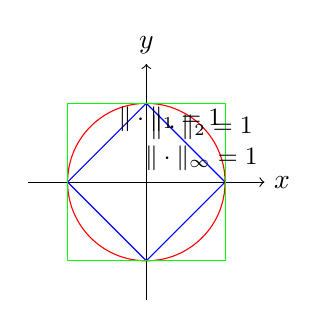
\begin{tikzpicture}
		% Coordinate system
		\draw[->] (-1.5,0) -- (1.5,0) node[right] {$x$};
		\draw[->] (0,-1.5) -- (0,1.5) node[above] {$y$};

		% Unit balls for different norms
		\draw[blue] (1,0) -- (0,1) -- (-1,0) -- (0,-1) -- cycle;
		\draw[red] (0,0) circle (1cm);
		\draw[green] (1,1) -- (1,-1) -- (-1,-1) -- (-1,1) -- cycle;

		\node at (0.7,0.7) {\small $\|\cdot\|_2=1$};
		\node at (0.3,0.8) {\small $\|\cdot\|_1=1$};
		\node at (0.7,0.3) {\small $\|\cdot\|_\infty=1$};
	\end{tikzpicture}
	\caption{Enhetskuler for forskjellige $p$-normer i $\mathbb{R}^2$. Enhver vektor på disse kurvene har norm lik 1. Blå: 1-norm (diamant). Rød: 2-norm (sirkel). Grønn: $\infty$-norm (kvadrat).}
	\label{fig:vector_norms}
\end{figure}

\subsubsection{Matrisenormer}

\begin{definition}{Matrisenorm}{matrix_norm}
	En matrisenorm på $\mathbb{R}^{m \times n}$ er en funksjon $\|\cdot\| : \mathbb{R}^{m \times n} \to \mathbb{R}$ som tilfredsstiller:
	\begin{enumerate}
		\item $\|A\| \geq 0$ for alle $A \in \mathbb{R}^{m \times n}$, og $\|A\| = 0$ hvis og bare hvis $A = 0$ (positivitet)
		\item $\|\alpha A\| = |\alpha| \cdot \|A\|$ for alle $A \in \mathbb{R}^{m \times n}$ og $\alpha \in \mathbb{R}$ (homogenitet)
		\item $\|A + B\| \leq \|A\| + \|B\|$ for alle $A,B \in \mathbb{R}^{m \times n}$ (trekantulikheten)
	\end{enumerate}
\end{definition}

En praktisk matrisenorm er Frobenius-normen, som måler matrisen som om den var en lang vektor:
\[
	\|A\|_F = \sqrt{\sum_{i=1}^m \sum_{j=1}^n |a_{ij}|^2} = \sqrt{\text{tr}(A^T A)}
\]

\subsection{Konsistente og underordnede matrisenormer}

\begin{definition}{Konsistent matrisenorm}{consistent_norm}
	En matrisenorm $\|\cdot\|$ på $\mathbb{R}^{n \times n}$ kalles konsistent (eller sub-multiplikativ) hvis
	\[
		\|AB\| \leq \|A\| \cdot \|B\|
	\]
	for alle $A, B \in \mathbb{R}^{n \times n}$.
\end{definition}

Denne egenskapen er viktig fordi den lar oss "ta ut" normen når vi har produkter av matriser, noe som er grunnleggende for mange konvergensbevis.

\begin{definition}{Underordnet matrisenorm}{subordinate_norm}
	Gitt en vektornorm $\|\cdot\|_v$ på $\mathbb{R}^n$, defineres den underordnede matrisenormen $\|\cdot\|_M$ på $\mathbb{R}^{n \times n}$ som
	\[
		\|A\|_M = \max_{\|x\|_v = 1} \|Ax\|_v = \max_{x \neq 0} \frac{\|Ax\|_v}{\|x\|_v}
	\]
\end{definition}

Intuitivt måler den underordnede normen den maksimale strekningen som matrisen $A$ kan påføre enhver enhetsvektor.

De vanligste underordnede matrisenormene er:
\begin{align*}
	\|A\|_1      & = \max_{1 \leq j \leq n} \sum_{i=1}^n |a_{ij}| \quad \text{(maksimal kolonnesum)} \\
	\|A\|_2      & = \sqrt{\lambda_{\max}(A^T A)} \quad \text{(største singulærverdi)}               \\
	\|A\|_\infty & = \max_{1 \leq i \leq n} \sum_{j=1}^n |a_{ij}| \quad \text{(maksimal radsum)}
\end{align*}

Disse normene er praktiske fordi de er relativt enkle å beregne og har direkte tolkninger.

\begin{theorem}{Egenskaper ved underordnede normer}{subordinate_properties}
	\begin{enumerate}
		\item Enhver underordnet matrisenorm er konsistent.
		\item For enhver matrise $A \in \mathbb{R}^{n \times n}$ og vektor $x \in \mathbb{R}^n$, gjelder
		      \[
			      \|Ax\|_v \leq \|A\|_M \cdot \|x\|_v
		      \]
	\end{enumerate}
\end{theorem}

\begin{figure}
	\centering
	\begin{tikzpicture}
		% Coordinate system
		\draw[->] (-3,0) -- (3,0) node[right] {$x$};
		\draw[->] (0,-3) -- (0,3) node[above] {$y$};

		% Unit circle
		\draw[blue] (0,0) circle (1cm);

		% Transformed ellipse (for matrix A)
		\draw[red, dashed] (0,0) ellipse (2cm and 0.5cm);

		% Labels
		\draw[|-|] (0,-1.5) -- (2,-1.5) node[midway,below] {$\|A\|_2$};

		\node at (0,3.5) {Visualisering av matrise-2-norm};
	\end{tikzpicture}
	\caption{Illustrasjon av 2-matrisenormen for en matrise $A$. Den blå sirkelen er enhetskulen i 2-norm, og den røde ellipsen er resultatet av å anvende $A$ på denne enhetskulen. Normen $\|A\|_2 = 2$ er den maksimale strekningen som $A$ påfører.}
	\label{fig:matrix_norm}
\end{figure}

\subsection{Matrisenormer og spektralradius}

\begin{definition}{Spektralradius}{spectral_radius}
	Spektralradiusen til en matrise $A \in \mathbb{C}^{n \times n}$ er definert som
	\[
		\rho(A) = \max\{|\lambda| : \lambda \text{ er en egenverdi av } A\}
	\]
	altså den største absoluttverdien av egenverdiene til $A$.
\end{definition}

Spektralradiusen er et fundamentalt mål på hvordan en matrise oppfører seg ved gjentatt anvendelse.

\begin{theorem}{Spektralradius og matrisenormer}{spectral_radius_norms}
	La $A \in \mathbb{C}^{n \times n}$ og $\|\cdot\|$ være en konsistent matrisenorm. Da gjelder:
	\begin{enumerate}
		\item $\rho(A) \leq \|A\|$
		\item For enhver $\varepsilon > 0$ finnes det en konsistent matrisenorm $\|\cdot\|_\varepsilon$ slik at $\|A\|_\varepsilon \leq \rho(A) + \varepsilon$
	\end{enumerate}
\end{theorem}

Dette betyr at spektralradiusen er den "best mulige nedre grense" for enhver konsistent matrisenorm.

\begin{theorem}{Konvergens av matrisepotenser}{matrix_power_convergence}
	La $A \in \mathbb{C}^{n \times n}$. Da gjelder følgende:
	\begin{enumerate}
		\item $\lim_{k \to \infty} A^k = 0$ hvis og bare hvis $\rho(A) < 1$
		\item For enhver konsistent matrisenorm $\|\cdot\|$, hvis $\|A\| < 1$, så er $\lim_{k \to \infty} A^k = 0$
	\end{enumerate}
\end{theorem}

Dette resultatet er ekstremt viktig i numerisk analyse, spesielt for å analysere konvergensen av iterative metoder.

\begin{figure}
	\centering
	\begin{tikzpicture}
		% Complex plane
		\draw[->] (-3,0) -- (3,0) node[right] {Re};
		\draw[->] (0,-3) -- (0,3) node[above] {Im};

		% Unit circle
		\draw[gray, dashed] (0,0) circle (1cm);

		% Eigenvalues inside unit circle
		\fill[blue] (0.5,0.1) circle (2pt) node[above right] {$\lambda_1$};
		\fill[blue] (-0.3,0.7) circle (2pt) node[above left] {$\lambda_2$};
		\fill[blue] (-0.3,-0.3) circle (2pt) node[below left] {$\lambda_3$};

		% Spectral radius (largest |λ|)
		\draw[red, ->, thick] (0,0) -- (-0.3,0.7);
		\node[red] at (1,1.5) {$\rho(A) = \max_i|\lambda_i| \approx 0.76$};

		\node at (0,-3.5) {Spektralradius og konvergens: $\rho(A) < 1 \implies \lim_{k \to \infty} A^k = 0$};
	\end{tikzpicture}
	\caption{Spektralradius og konvergens. Når alle egenverdiene ligger innenfor enhetssirkelen ($\rho(A) < 1$), konvergerer sekvensen $A^k$ mot nullmatrisen når $k \to \infty$. Dette er grunnleggende for stabilitetsanalyse av iterative metoder.}
	\label{fig:spectral_radius}
\end{figure}

\section{Normer og indre produkt}
\subsection{Normer}
Normer i funksjonsrom utvider konseptet med vektornormer til uendeligdimensjonale rom. De måler "størrelsen" eller "lengden" av funksjoner.

\subsection{Indre produkt}
\begin{definition}{Indreprodukt av funksjoner i $\mathrm{L}^2$ (Skalarprodukt)}{L2_inner_product}
	Hilbertrommet $\Lrm^2$ er gitt ved operasjonen $(\Lrm_2, \inner{,}_{2})$ hvor $\Lrm_2$ er settet av alle funksjoner som oppfyller:
	\[
		\int_{-\infty}^{\infty} |f(x)|^2 \,dx < \infty
	\]
	og vi har for $v, w\in \Lrm_2$
	\[
		\inner{v,w}_w = \int_\Omega v(x)w(x) \,dx
	\]
	hvor $\Omega = [a, b]$, er et endelig intervall.
\end{definition}

Dette indre produktet gir oss en måte å måle "overlappen" eller "likheten" mellom to funksjoner. Intuitivt, jo større indreprodukt, desto mer "like" er funksjonene. Hvis indreproduktet er null, kalles funksjonene ortogonale, noe som betyr at de ikke har noen "overlapp" i denne forstand.

Et viktig eksempel er Fourier-analysens bruk av indreprodukt for å måle hvor mye en funksjon "inneholder" av ulike frekvenskomponenter.

\section{Funksjonsrom}
Funksjonsrom er samlinger av funksjoner med bestemte egenskaper. De danner grunnlaget for å analysere differensialligninger i en generalisert ramme.

\paragraph{Funksjonsrommet \(V\)} Rommet av funksjoner som tilfredsstiller randbetingelsene.
\[ V = \{ v \in C^2(\Omega) \, | \, v(a) = \alpha, v(b) = \beta \} \]
Dette rommet representerer alle mulige funksjoner som kan være løsninger på problemet vårt.

\paragraph{Testfunksjoner \(v(x)\)} Funksjoner i \(V\) som brukes til å formulere den svake formen.
Testfunksjoner lar oss "teste" en mulig løsning ved å integrere mot disse funksjonene.

\paragraph{Basisfunksjoner \(\phi_i(x)\)} Lokale funksjoner som spenner ut løsningsrommet.
\begin{itemize}
	\item Har kompakt støtte (er null utenfor et lite område)
	\item Oppfyller \(\phi_i(x_j) = \delta_{ij}\) (Kronecker delta)
\end{itemize}

Basisfunksjoner er byggesteinene vi bruker til å konstruere numeriske løsninger. I endelig element-metoden er disse typisk "hatt-funksjoner" eller polynomer som er positive i små områder og null ellers.

\begin{lemma}{Fundamental lemma of calculus of variations}{fundlemma}
	La $\Omega \subset \mathbb{R}^n$ være et åpent område med regulær rand og $f: \Omega \rightarrow \mathbb{R}$ være en kontinuerlig funksjon.
	Hvis
	\begin{equation}
		\int_{\Omega} \omega(x) \varphi(x) \, dx = 0
	\end{equation}
	holder for alle $\varphi \in \Ccal_c^{\infty}(\Omega)$ (dvs. uendelig differensierbare funksjoner med kompakt støtte i $\Omega$), da er $\omega(x) = 0$ for alle $x \in \Omega$.
\end{lemma}

Dette lemmaet er grunnleggende for variasjonelle formuleringer av differensialligninger. Det forteller oss at hvis integralet av et produkt er null for alle testfunksjoner, så må funksjonen selv være null nesten overalt.

\subsection{Energifunksjoner}
La \(F: V \mapsto \mathbb{R}\) være en funksjon som tar inn en funksjon \(v\) og gir ut et reelt tall. Energien til en funksjon \(v\) er gitt ved:
\[
	F(v) = \frac{1}{2} \langle v, v \rangle - \langle f, v \rangle
\]

I mange fysiske problemer representerer dette faktisk den fysiske energien i systemet. Minimering av denne energifunksjonen gir oss løsningen på det tilsvarende differensialligningsmessige problemet, noe som er bakgrunnen for variasjonelle formuleringer.

\section[Sobolev-rom]{Sobolev-rom \(H^1(\Omega)\)}
Sobolev-rom er funksjonsrom som er spesielt tilpasset for å jobbe med partiell-deriverte differensialligninger.

\begin{equation}
	H^1(\Omega) = \{ v \in L^2(\Omega) : \nabla v \in L^2(\Omega) \}
\end{equation}

Dette er rommet av kvadratisk integrerbare funksjoner som også har kvadratisk integrerbare deriverte. I motsetning til $C^1$-funksjoner, trenger Sobolev-funksjoner ikke være kontinuerlig differensierbare i vanlig forstand - de kan ha "svake" deriverte som eksisterer i en mer generalisert betydning.

\begin{definition}{Sobolev-rom $\mathcal{H}_0^1(\Omega)$}{sob_space}
	La $u:\overset{\subseteq \R^d}{\Omega} \to \R$ være en funksjon, med $u, \nabla u \in L^2(\Omega)$.

	\begin{equation}
		\norm*{u}_{\mathcal{H}^1(\Omega)}^2 = \norm*{u}_{L^2(\Omega)}^2 + \norm*{\nabla u}_{L^2(\Omega)}^2
		= \int_\Omega \abs{u}^2 \, dx + \int_\Omega \abs{\nabla u}^2 \, dx
	\end{equation}
	\begin{equation}
		\mathcal{H}_0^1(\Omega) = \{u \in \mathcal{H}^1(\Omega) \mid u = 0 \text{ på } \partial \Omega\}
	\end{equation}

	Med andre ord, en funksjon $u$ er i $\mathcal{H}^1_0(\Omega)$ hvis:
	\begin{itemize}
		\item $u$ og $\nabla u$ er kvadratisk integrerbare i $H^1(\Omega)$
		      \begin{equation}
			      \norm*{u}_{L^2(\Omega)}^2 = \int_\Omega \abs{u}^2 \, dx < \infty \quad \text{og} \quad \norm*{\nabla u}_{L^2(\Omega)}^2 = \int_\Omega \abs{\nabla u}^2 \, dx < \infty
		      \end{equation}
		\item $u$ er lik null på randen $\partial \Omega$ av domenet $\Omega$
		      \begin{equation}
			      u(x) = 0 \quad \forall x \in \partial \Omega
		      \end{equation}
	\end{itemize}
\end{definition}

Rommet $H^1_0(\Omega)$ er spesielt viktig for differensialligninger med Dirichlet-grensebetingelser, der løsningene er spesifisert på randen.

\begin{equation}
	V := H^1_0(\Omega) = \{ v \in H^1(\Omega) : v = 0 \text{ på } \partial\Omega \}
\end{equation}

\section{Svake deriverte og Variasjonell formulering}
\subsection{Svake deriverte}
Svake deriverte er en generalisering av vanlige deriverte som tillater oss å jobbe med funksjoner som ikke nødvendigvis er glatte i vanlig forstand.

Idéen bak svake deriverte er å definere den deriverte av en funksjon basert på hvordan den oppfører seg i integraler mot testfunksjoner, snarere enn ved grenseverdier av differenskvotienter.

Dette konseptet er essensielt for å håndtere problemer hvor løsninger kan ha diskontinuiteter eller singulariteter, noe som er vanlig i mange fysiske problemer.

\subsection{Variasjonell formulering}
Variasjonell formulering er en teknikk for å omformulere en differensialligning som et variasjonsproblem, der løsningen minimerer en viss energifunksjonell eller tilfredsstiller en svak form av den originale ligningen.

For en typisk annen ordens differensialligning:
\begin{equation}
	-\nabla \cdot (a(x) \nabla u) + c(x)u = f(x) \quad \text{i } \Omega
\end{equation}
med Dirichlet-grensebetingelser $u = 0$ på $\partial\Omega$, er den svake formuleringen:

Finn $u \in H^1_0(\Omega)$ slik at
\begin{equation}
	\int_\Omega a(x) \nabla u \cdot \nabla v \, dx + \int_\Omega c(x) u v \, dx = \int_\Omega f(x) v \, dx \quad \forall v \in H^1_0(\Omega)
\end{equation}

Denne formuleringen krever mindre glatthet av løsningen $u$ og er utgangspunktet for finite element-metoden.

\subsection{Bilinær form}
\begin{definition}{Bilinær form}{bilinear_form}
	En bilinær form $a: V \times V \to \mathbb{R}$ er en funksjon som er lineær i begge argumentene, dvs. for alle $u,v,w \in V$ og $\alpha, \beta \in \mathbb{R}$ gjelder:
	\begin{align*}
		a(\alpha u + \beta v, w) & = \alpha a(u,w) + \beta a(v,w)  \\
		a(u, \alpha v + \beta w) & = \alpha a(u,v) + \beta a(u,w).
	\end{align*}
\end{definition}

For eksempel i Poisson-ligningen blir den bilinære formen:
\begin{equation}
	a(u,v) = \int_\Omega \nabla u \cdot \nabla v \, dx
\end{equation}

Bilinære former er byggeklossene i variasjonelle formuleringer og representerer typisk energien eller arbeidet i det fysiske systemet.

\subsection{Lax-Milgram teoremet}\label{sec:lax_milgram}
Lax-Milgram-teoremet er et fundamentalt resultat som garanterer eksistens og entydighet av løsninger til variasjonelle problemer under visse betingelser.

\begin{theorem}{Lax-Milgram}{lax_milgram}
	La $V$ være et Hilbert-rom, og la $a: V \times V \to \mathbb{R}$ være en bilinær form som er \emph{kontinuerlig} og \emph{koersiv}. Anta at $F: V \to \mathbb{R}$ er en begrenset lineær funksjonell. Da finnes det en entydig løsning $u \in V$ slik at
	\[
		a(u,v) = F(v) \quad \forall v \in V.
	\]
\end{theorem}

For at teoremet skal gjelde, må bilinærformen $a(\cdot, \cdot)$ oppfylle to viktige egenskaper:

\paragraph{Kontinuitet} Det finnes en konstant $M > 0$ slik at
\[
	|a(u,v)| \leq M\, \|u\|_V\, \|v\|_V \quad \text{for alle } u,v\in V.
\]
Dette betyr at små endringer i inngangsfunksjonene resulterer i små endringer i bilinærformen.

\paragraph{Koersivitet} Det finnes en konstant $\alpha > 0$ slik at
\[
	a(v,v) \geq \alpha\, \|v\|_V^2 \quad \text{for alle } v\in V.
\]
Dette er en slags "positiv definitthet" for bilinærformen og sikrer at problemet er velposert.

Når $F$ er en begrenset lineær funksjonell på $V$ (altså $F \in V'$), garanterer teoremet at:
\begin{itemize}
	\item Det finnes en entydig løsning $u \in V$ til variasjonsproblemet
	      \[
		      a(u,v)=F(v) \quad \text{for alle } v\in V.
	      \]

	\item Løsningen oppfyller den stabile estimeringen
	      \[
		      \|u\|_V \leq \frac{1}{\alpha}\, \|F\|_{V'}.
	      \]
	      Dette betyr at løsningen avhenger kontinuerlig av dataene, en viktig egenskap for numeriske metoder.
\end{itemize}

\subsection*{Galerkins ortogonalitet}

\begin{definition}{Galerkins Ortogonalitet}{galerkins_ortogonalitet}
	\[
		a(u - u_h, v) = 0 \quad \forall v \in V_h
	\]
	hvor $u_h$ er den approksimerte løsningen, $u$ er den eksakte løsningen, og $V_h$ er det endelige elementrommet.
\end{definition}

Galerkins ortogonalitet betyr at feilen $u - u_h$ er "ortogonal" til hele approksiamasjonsrommet $V_h$ med hensyn til bilinærformen $a(\cdot,\cdot)$. Dette er en fundamental egenskap ved Galerkins metode, og betyr at approksiamasjonen $u_h$ er optimal i en viss forstand.

\subsection{Céas lemma}
Céas lemma gir en øvre grense for feilen i Galerkin-approksimasjoner og er et viktig verktøy for å analysere konvergens av endelig element-metoder.

\begin{lemma}{Céas lemma}{ceas_lemma}
	\[
		\norm*{u - u_h} \leq \frac{M}{\alpha} \inf_{v \in V_h} \norm*{u - v}
	\]
	hvor $M$ er kontinuitetskonstanten for bilinærformen $a(\cdot, \cdot)$, og $\alpha$ er koersivitetskonstanten.
\end{lemma}

Dette lemmaet forteller oss at feilen i den numeriske løsningen $u_h$ er begrenset av den best mulige approksimasjonen av den eksakte løsningen $u$ i rommet $V_h$, multiplisert med forholdet $\frac{M}{\alpha}$.

Dette er et kraftig resultat fordi det lar oss fokusere på approksiamasjonsegenskapene til rommet $V_h$ når vi analyserer konvergensen av endelig element-metoder. For eksempel, hvis vi vet at $V_h$ består av stykkevis lineære funksjoner, kan vi bruke klassisk approksimasjonsteori til å vise at $\inf_{v \in V_h} \norm*{u - v} = O(h^2)$ når $u$ er glatt nok, og dermed at $\norm*{u - u_h} = O(h^2)$.